All have 15 responses unless otherwise stated. Numbers in brackets are the number of participants with that answer.

\begin{figure}[H]
\begin{tikzpicture}
\pie[radius=2, text = legend]{93.3/18-30 (14), 6.7/Under 18 (1)}
\end{tikzpicture}
\caption{What is your age?}
\end{figure}

\begin{figure}[H]
\begin{tikzpicture}
\pie[radius=2, text = legend]{60/A Level Standard (9), 33.3/Degree Level Standard (5), 6.7/GCSE Level Standard (1)}
\end{tikzpicture}
\caption{What is your mathematical ability?}
\end{figure}

\begin{figure}[H]
\begin{tikzpicture}
\pie[radius=2, text = legend]{66.7/No (10), 33.3/Yes \,I have a basic understanding (5)}
\end{tikzpicture}
\caption{Have you used Natural Deduction logic prior to playing the game?}
\end{figure}

\begin{figure}[H]
\begin{tikzpicture}
\pie[radius=2, text = legend]{13.3/No (2), 86.7/Yes (13)}
\end{tikzpicture}
\caption{Do you think you have learnt more about Natural Deduction as a result of playing the game?}
\end{figure}

\begin{figure}[H]
\begin{tikzpicture}
\pie[radius=2, text = legend]{0/No (0), 100/Yes (15)}
\end{tikzpicture}
\caption{Did you do the tutorial at the start of the game?}
\end{figure}

\begin{figure}[H]
\begin{tikzpicture}
\pie[radius=2, text = legend]{0/No (0), 100/Yes (15)}
\end{tikzpicture}
\caption{If you answered Yes, did you complete the tutorial?}
\end{figure}

\begin{figure}[H]
\begin{tikzpicture}
\pie[radius=2, text = legend]{0/No (0), 100/Yes (15)}
\end{tikzpicture}
\caption{If you answered Yes, did you find the tutorial useful?}
\end{figure}

\begin{figure}[H]
\begin{tikzpicture}
\pie[radius=2, text = legend]{0/No (0), 100/Yes (15)}
\end{tikzpicture}
\caption{Did you use the hints button during the game?}
\end{figure}

\begin{figure}[H]
\begin{tikzpicture}
\pie[radius=2, text = legend]{33.3/No (5), 66.7/Yes (10)}
\end{tikzpicture}
\caption{If Yes to using hints, did you find them useful?}
\end{figure}

\begin{figure}[H]
\begin{tikzpicture}
\pie[radius=2, text = legend]{20/Completed the game (Finished level 6) (3), 6.7/Level 6 (1), 13.3/Level 5 (2), 6.7/Level 4 (1), 20/Level 3 (3), 33.3/Level 2 (5), 0/Level 1 (0)}
\end{tikzpicture}
\caption{Which level of the game did you get to?}
\end{figure}

\begin{figure}[H]
\begin{tabular}{|p{12cm}|} 
\hline
I got frustrated with the proof! I knew what I wanted it to look like but I kept doing it wrong the proofs kept getting placed on the wrong dots from where I wanted them. \\
\hline
It took me a while to create a proof and then it was wrong and I couldn't be bothered to create it all again from scratch \\
\hline
could not work out how to complete the level correctly \\
\hline
Couldn't answer Question 2, as I have no idea what proof it is wanting or how to prove it \\
\hline
Because I was watching Big Bang Theory :) \\
\hline
Time constraints. \\
\hline
Not enough knowledge of proofs or time \\
\hline
Time consuming \\
\hline
Conjunction elimination is poorly explained, I dont understand what I should be doing what so ever \\
\hline
\end{tabular}
\caption{If you didn't finish the game, why not?}
\end{figure}

\begin{figure}[H]
\begin{tabular}{|p{12cm}|} 
\hline
Yes \\
\hline
Levels increased nicely \\
\hline
Thought level 2 got too difficult too quickly, there should have been an example to show how to put an extra 2 top 1 bottom in to prove the whole thing \\
\hline
Very well \\ 
\hline
Good curve \\
\hline
found level 2 a lot harder than 1 \\
\hline
The difficulty increased quickly for a novice \\
\hline
Yes, the difficulty increased. \\
\hline
Yes checked internet for more info \\
\hline
Not really but maybe it would for the last 2 \\
\hline
Exponentially \\
\hline
definitely \\
\hline
First 2 levels were easy, level 3 made no sense, so I guess there was a difficulty curve \\
\hline
Yes, difficulty increased as game progressed but not too quickly, just the right amount. \\
\hline
\end{tabular}
\caption{How did you feel the difficulty curve increase as the game progressed? (Did the difficulty of the levels increase as the game went on?)}
\end{figure}

\begin{figure}[H]
\begin{tabular}{|p{12cm}|} 
\hline
Minimalistic design \\
\hline
Drag and drop capability \\
\hline
The duplicate option! (when it worked) \\
\hline
Though provoking but logical \\
\hline
Colours \\ 
\hline
allows you to think logically and it is interactive \\
\hline
Good user interface \\
\hline
Tutorial explained the concepts of the game well \\
\hline
Simplicity \\
\hline
You can assemble your answer \\
\hline
It let you work things out yourself \\
\hline
The challenge \\
\hline
i distracted me from my work, like all good games \\
\hline
Nice drag and drop stuff that is mostly smooth, at times there are issues with item selection. \\
\hline
Mind puzzle / brain-teaser type game \\
\hline
\end{tabular}
\caption{What did you like most about the game?}
\end{figure}

\begin{figure}[H]
\begin{tabular}{|p{12cm}|} 
\hline
no \\
\hline
no \\
\hline
No major issues, but it caused chrome to hog a lot of memory and processing power \\
\hline
i couldn't undo an action when i did something wrong so i had to bin the whole thing and start again \\
\hline
For complicated proofs it was so frustrating when I had done somethign wrong there was no undo button / i couldnt drag the letter back out again!! I did this on every single level. Level 4 I put A on top of A, and it said proof incorrect- check A. I Know this is meant to help the user but it wasnt very helpful!! Maybe saying "the top A" would have been better. I didnt understand why a should be on top of b in the implication bit, it didnt seem to work like that in the game \\
\hline
Not really \\
\hline
No \\
\hline
Couldn't answer it, still don't know how to proceed and the hints are just confusing \\
\hline
Apart from my lack of knowledge, no \\
\hline
Size of game to fit the browser required zooming out as forewarned. \\
\hline
yes \\
\hline
It was annoying having to delete everything and start again if something was in the wrong place \\
\hline
My answer at the end wasn't accepted even though it should be right, I just didn't write it in the 'correct' way \\
\hline
Drag and drop issues, poor explanations. removing items from a structure would also have been useful, I found myself creating large structures and then having to bin them, rather than tweak them. \\
\hline
Small bugs \\
\hline
\end{tabular}
\caption{Did you have any problems whilst playing the game?}
\end{figure}

\begin{figure}[H]
\begin{tabular}{|p{12cm}|} 
\hline
No \\
\hline
No \\
\hline
No \\
\hline
no \\
\hline
no \\
\hline
Potentially fairly resource intensive, but nothing major \\
\hline
\% signs in my incorrect message \\
\hline
Not yet \\
\hline
No. \\
\hline
see notes \\
\hline
I don't know whether this is a bug but it didn't accept the answer was right if the parts were in the wrong order \\
\hline
Didn't show me an image in the hints (some overlap of writing?) \\
\hline
"something wrong with undefined..?" on level six, the hint didnt appear for some reason, so i had to use the hint and lose point even though i hadnt actually seen it before the level as intended. \\
\hline
Not that I know of. \\
\hline
Some of the pictures did not show up \\
\hline
\end{tabular}
\caption{Did you find any bugs in the code?}
\end{figure}

\begin{figure}[H]
\begin{tabular}{|p{12cm}|} 
\hline
Mobile compatibility is a must, which this currently doesn't support well. Laptop/desktop personal computing is in decline - this really should be touchscreen compatible. \\
\hline
An 'undo' button to take back the last step. Dragging straight from the button set instead of pressing and then dragging in the canvas. \\
\hline
When you click a button make the object go onto the canvas at the bottom above the button to make it easier to use straight away. Also, brackets could be another object dragged onto stuff, dragging the object onto the brackets was a bit strange when the rest isnt like that. Red outline when deleting something might be clearer than blue? I didn't know how I was losing points, the user isnt told how points are given out at all. Delete all button next to check proof, noooooo! My beautiful long proof! When hovering a proof over a dot, it would be useful for the underneath part to be expanded to fit my on top proof in- I ended up putting stuff in the wrong place because I thought it was over one dot when actually it wasnt at all \\
\hline
It would be nice if you could detach objects (like A, B, etc.) instead of having to delete it and start over everytime you make a mistake \\
\hline
Display the rules \\
\hline
be able to undo once you have put two parts together \\
\hline
It might be useful to have an undo button, make it all fit on the screen so you can't scroll \\
\hline
Zoom thing / Undo / novice tutorial \\
\hline
Reduction of the game size? As some potential users, younger or older, may be unaware on adjusting browser size. \\
\hline
see notes \\
\hline
The controls could be easier \\
\hline
More explanations \\
\hline
a copy button? less white space on terms the larger they get. \\
\hline
Better explanations, the ability to tweak current proofs, a better hint system that gives you a hint in to how the structure should be. For exa,ple, if the hint actually shown me how to do level 3, I may then have understood what was going on. I also found myself clicking the buttons at the bottom and trying to drag items from there, that was a possible usability issue. \\
\hline
Allow proofs (2 top/ 1 bottom etc) to be duplicated \\
\hline
\end{tabular}
\caption{What improvements do you think could be made to the game?}
\end{figure}

\begin{figure}[H]
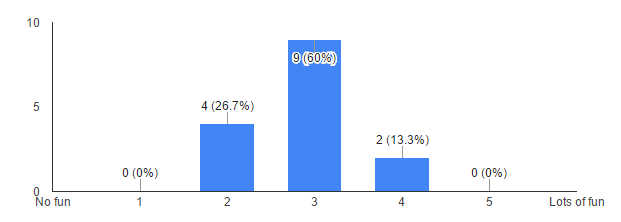
\includegraphics[scale=0.8]{fun}
\caption{How fun did you find the game?}
\end{figure}

\begin{figure}[H]
\begin{tabular}{|p{12cm}|} 
\hline
I'm not hugely interested in maths, nor particularly good at it! I'm sure my opinion is no reflection on how good the game is for those who are! \\
\hline
There's only so much fun you can find maths. \\
\hline
I found it really engaging because I wanted to keep going and reach more levels and complete the proofs and learn more rules, but the usability issues were really frustrating and it took me a long time to construct the proof for level 5 which I then did wrong because I misplaced one part of it. Starting again would have been frustrating so I stopped then. \\
\hline
Trying to solve the problems was fun but it was tedious to have to scroll down the screen to create the buttons each time and remake everything from scratch when an error was made \\
\hline
Fiddly to input new formulas \\
\hline
found it hard \\
\hline
Ew, maths \\
\hline
Game seems education orientated. \\
\hline
Satisfaction when got the answer. Alot of trial and error \\
\hline
It was quite good but it's still doing proofs which are boring \\
\hline
ew maths \\
\hline
Didn't get far enough to appreciate it, it also took far too long to move items around, hindering the fun. \\
\hline
\end{tabular}
\caption{Give a reason for your answer...}
\end{figure}

\begin{figure}[H]
\begin{tikzpicture}
\pie[radius=2, text = legend]{15.4/No (2), 84.6/Yes (11)}
\end{tikzpicture}
\caption{Do you think that playing this game is a better way to learn than learning in traditional methods? (E.g. Pen and paper/ Lectures/ Classroom session) (13 Responses)}
\end{figure}

\begin{figure}[H]
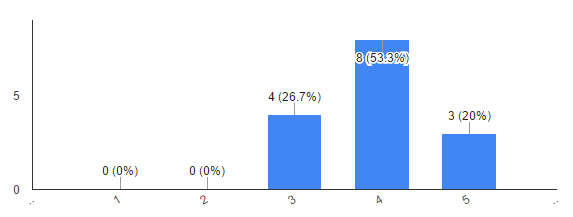
\includegraphics[scale=0.8]{education}
\caption{As an educational tool, how effective do you feel the game is?}
\end{figure}

\begin{figure}[H]
\begin{tabular}{|p{12cm}|} 
\hline
Perhaps add in a 'reveal answer' button if the question is too hard and the user can't figure out the answer. \\
\hline
It's much more fun than learning from a book or in a lecture! \\
\hline
I don't think the hints were really "hints" they were more "these are the definitions for the techniques", I think they should be displayed on the screen the entire time and hints should tell you how to go about completing the level \\
\hline
Still not sure what Natural Deduction is \\
\hline
\end{tabular}
\caption{Any other comments...}
\end{figure}
